% !TEX TS-program = pdflatex
% !TEX encoding = UTF-8 Unicode
% !TEX spellcheck = es_CL

% This is a simple template for a LaTeX document using the "article" class.
% See "book", "report", "letter" for other types of document.

\documentclass[11pt]{article} % use larger type; default would be 10pt

\usepackage{svn-multi}
%\svnidlong
%{$HeadURL$}
%{$LastChangedDate$}
%{$LastChangedRevision$}
%{$LastChangedBy$}
\usepackage[utf8]{inputenc} % set input encoding (not needed with XeLaTeX)
\usepackage[T1]{fontenc}
\usepackage{lmodern}
\usepackage[spanish,es-tabla]{babel}
\spanishdecimal{.}
%%% Examples of Article customizations
% These packages are optional, depending whether you want the features they provide.
% See the LaTeX Companion or other references for full information.

%%% PAGE DIMENSIONS
\usepackage{geometry} % to change the page dimensions
\geometry{letterpaper} % or letterpaper (US) or a5paper or....
\geometry{margin=1.4in} % for example, change the margins to 2 inches all round
% \geometry{landscape} % set up the page for landscape
%   read geometry.pdf for detailed page layout information

\usepackage{graphicx} % support the \includegraphics command and options

% \usepackage[parfill]{parskip} % Activate to begin paragraphs with an empty line rather than an indent

%%% PACKAGES
\usepackage{booktabs} % for much better looking tables
\usepackage{array} % for better arrays (eg matrices) in maths
\usepackage{paralist} % very flexible & customisable lists (eg. enumerate/itemize, etc.)
\usepackage{verbatim} % adds environment for commenting out blocks of text & for better verbatim
\usepackage[subrefformat=parens,labelformat=parens]{subfig} % make it possible to include more than one captioned figure/table in a single float
% These packages are all incorporated in the memoir class to one degree or another...

%\usepackage{amsmath}
\usepackage{mathtools}
\usepackage{amsfonts}


% Paquetes adicionales
\usepackage{siunitx}
\sisetup{load=derived} % loading \si
\usepackage{xcolor}
\usepackage{multicol}
% Paquete titling permite reducir el margen superior
%\usepackage{titling}
%\setlength{\droptitle}{-10ex}
%\usepackage{enumitem}
% agrega la opcion H a las figuras para que queden donde uno quiere
%\usepackage{float}
%\usepackage{microtype}

% Fuentes
% MinionPro
%\usepackage[minionint,textlf,mathlf]{MinionPro}
% Fijar fuente Sans Serif  a Myriad
%\renewcommand{\sfdefault}{Myriad-LF}
%\usepackage[T1]{fontenc}

% Fuente similar a Times New Roman
%\usepackage{tgtermes}
%\usepackage[T1]{fontenc}

%\usepackage{utopia} % Cambia solo la fuente del texto
%\usepackage[urw-garamond]{mathdesign} %Problemas con wrapfig
%\usepackage[utopia]{mathdesign} %Problemas con wrapfig
%\usepackage[charter]{mathdesign} % HERMOSO!!
%\usepackage{fourier} % Problemas con wrapfig
%% Fuente palatino
\usepackage[T1]{fontenc}
\usepackage[sc]{mathpazo}
\linespread{1.05}
%% Similar a palatino pero extendida
%\usepackage{tgpagella}
%\usepackage[T1]{fontenc}
%\usepackage[scaled=0.86]{berasans}
%
%\usepackage{libertine-type1}% NICE!!
%\usepackage{libertine}
%\usepackage[ttscale=0.875]{libertine}
% La fuente typewriter de libertine es fea, asi que hay que cambiarla
%\usepackage{inconsolata}
%\usepackage[scaled=0.83]{beramono}
%\usepackage{DejaVuSansMono}
%\renewcommand\ttdefault{lmtt} % lmtt
%\usepackage[libertine]{newtxmath}
%\usepackage[T1]{fontenc}

%\usepackage[math]{iwona}
%\usepackage{fourier}

%\renewcommand{\sfdefault}{phv}
%\renewcommand{\sfdefault}{lmss} % Fuente por defecto en latex o cmss
% Fuente times
%\usepackage{newtxtext,newtxmath}


% Agregar directorio donde buscar figuras
\graphicspath{{./figuras/}}

%%% HEADERS & FOOTERS
\usepackage{fancyhdr} % This should be set AFTER setting up the page geometry
\pagestyle{fancy} % options: empty , plain , fancy
\renewcommand{\headrulewidth}{0pt} % customise the layout...
\lhead{}\chead{}\rhead{}
\lfoot{}\cfoot{\thepage}\rfoot{}

%%% SECTION TITLE APPEARANCE
%\usepackage{sectsty}
%\allsectionsfont{\sffamily\mdseries\upshape} % (See the fntguide.pdf for font help)
% (This matches ConTeXt defaults)

%%% ToC (table of contents) APPEARANCE
%\usepackage[nottoc,notlof,notlot]{tocbibind} % Put the bibliography in the ToC
%\usepackage[titles,subfigure]{tocloft} % Alter the style of the Table of Contents
%\renewcommand{\cftsecfont}{\rmfamily\mdseries\upshape}
%\renewcommand{\cftsecpagefont}{\rmfamily\mdseries\upshape} % No bold!

%%% END Article customizations

%%% The "real" document content comes below...

\title{Filtros}
\author{Fabián Inostroza}
%\date{} % Activate to display a given date or no date (if empty),
         % otherwise the current date is printed 


\usepackage{hyperref}
\hypersetup{
%    bookmarks=true,         % show bookmarks bar?
    unicode=false,          % non-Latin characters in Acrobat’s bookmarks
%    pdftoolbar=true,        % show Acrobat’s toolbar?
%    pdfmenubar=true,        % show Acrobat’s menu?
    pdffitwindow=false,     % window fit to page when opened
    pdfstartview={FitH},    % fits the width of the page to the window
    pdftitle={Filtros, filtro, complementario, complementary, filter, mpu6050, tilt, angle, ángulo, inclinación},    % title
    pdfauthor={Fabián Inostroza},     % author
%    pdfsubject={Subject},   % subject of the document
%    pdfcreator={Creator},   % creator of the document
%    pdfproducer={Producer}, % producer of the document
%    pdfkeywords={keyword1} {key2} {key3}, % list of keywords
    pdfnewwindow=true,      % links in new window
    colorlinks=true,       % false: boxed links; true: colored links
    linkcolor=blue,          % color of internal links (change box color with linkbordercolor)
    citecolor=green,        % color of links to bibliography
    filecolor=magenta,      % color of file links
    urlcolor=cyan           % color of external links
}

\begin{document}
\maketitle

\section{Aproximación discreta de función de transferencia continua}
Se usará integración numérica, el método de Euler.
La función de transferencia continua de un integrador es
\[ H(s) = \frac{1}{s}. \]
En el método de Euler se aproxima la integral con la siguiente 
ecuación
\[ y(k) = y(k-1)+ u(k)\cdot T_0 \]
donde \( y(k) \) es el valor de integral al paso \( k \),
\( u_k \) es la variable a integrar y \( T_0 \) es el 
tiempo de muestreo. Aplicando la transformada Z a la ecuación 
anterior se obtiene la siguiente función de transferencia
\[ H(z) = \frac{T_0}{1-z^{-1}} = \frac{1}{ \frac{1-z^{-1}}{T_0} } \]

Comparando la función de transferencia continua con la 
discreta se ve que se puede aproximar la función de 
 transferencia continua haciendo el reemplazo 
\begin{equation}
s = \frac{1-z^{-1}}{T_0} \label{eq:s2z}
\end{equation}.
 
\section{Filtro pasa bajos}
La versión circuital de un filtro pasa bajos se muestra en la Figura~\ref{fig:LPF}.

\begin{figure}[h!tb]
\centering
% XCircuit output "LP.tex" for LaTeX input from LP.ps
\def\putbox#1#2#3#4{\makebox[0in][l]{\makebox[#1][l]{}\raisebox{\baselineskip}[0in][0in]{\raisebox{#2}[0in][0in]{\scalebox{#3}{#4}}}}}
\def\rightbox#1{\makebox[0in][r]{#1}}
\def\centbox#1{\makebox[0in]{#1}}
\def\topbox#1{\raisebox{-0.60\baselineskip}[0in][0in]{#1}}
\def\midbox#1{\raisebox{-0.20\baselineskip}[0in][0in]{#1}}
   \scalebox{1}{
   \normalsize
   \parbox{2.20312in}{
   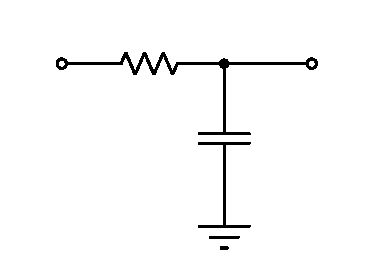
\includegraphics[scale=1]{LP}\\
   % translate x=447 y=332 scale 0.38
   \putbox{1.59in}{0.79in}{1.20}{\midbox{$C$}}%
   \putbox{0.88in}{1.41in}{1.20}{\centbox{$R$}}%
   \putbox{0.30in}{1.04in}{1.20}{\centbox{$V_{in}$}}%
   \putbox{1.97in}{1.04in}{1.20}{\centbox{$V_{out}$}}%
   } % close 'parbox'
   } % close 'scalebox'
   \vspace{-\baselineskip} % this is not necessary, but looks better

\caption{Filtro pasa bajos análogo.}
\label{fig:LPF}
\end{figure}

La función de transferencia de este filtro es
\[ H(s) = \frac{1}{RCs+1} = \frac{\omega_c}{s+\omega_c} \]

Usando \eqref{eq:s2z} se obtiene

\[ H(z) = \frac{\omega_c}{(1-z^{-1})/T_0 + \omega_c} \]
Aplicando transformada Z inversa se obtiene
\begin{align*}
y(k) &= \frac{1/T_0}{1/T_0+\omega_c}y(k-1) + 
\frac{\omega_c}{1/T_0+\omega_c} u(k)  \\
	&= (1-\alpha)y(k-1) + \alpha u(k)
\end{align*}
donde
\[ \alpha = \frac{\omega_c}{1/T_0+\omega_c} \]

\section{Filtro pasa altos}
La versión circuital de un filtro pasa altos se muestra en la Figura~\ref{fig:HPF}.

\begin{figure}[h!tb]
\centering
% XCircuit output "HP.tex" for LaTeX input from HP.ps
\def\putbox#1#2#3#4{\makebox[0in][l]{\makebox[#1][l]{}\raisebox{\baselineskip}[0in][0in]{\raisebox{#2}[0in][0in]{\scalebox{#3}{#4}}}}}
\def\rightbox#1{\makebox[0in][r]{#1}}
\def\centbox#1{\makebox[0in]{#1}}
\def\topbox#1{\raisebox{-0.60\baselineskip}[0in][0in]{#1}}
\def\midbox#1{\raisebox{-0.20\baselineskip}[0in][0in]{#1}}
   \scalebox{1}{
   \normalsize
   \parbox{2.20312in}{
   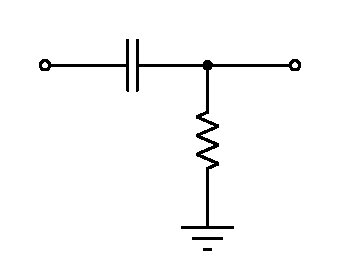
\includegraphics[scale=1]{HP}\\
   % translate x=447 y=332 scale 0.38
   \putbox{0.88in}{1.54in}{1.20}{\centbox{$C$}}%
   \putbox{1.47in}{0.79in}{1.20}{\midbox{$R$}}%
   \putbox{0.30in}{1.04in}{1.20}{\centbox{$V_{in}$}}%
   \putbox{1.97in}{1.04in}{1.20}{\centbox{$V_{out}$}}%
   } % close 'parbox'
   } % close 'scalebox'
   \vspace{-\baselineskip} % this is not necessary, but looks better

\caption{Filtro pasa altos análogo.}
\label{fig:HPF}
\end{figure}

La función de transferencia de este filtro es
\[ H(s) = \frac{RCs}{RCs+1} = \frac{s}{s+\omega_c} \]

Usando \eqref{eq:s2z} se obtiene

\[ H(z) = \frac{(1-z^{-1})/T_0}{(1-z^{-1})/T_0 + \omega_c} \]
Aplicando transformada Z inversa se obtiene
\begin{align*}
y(k) &= \frac{1/T_0}{1/T_0+\omega_c} y(k-1) + \frac{1/T_0}{1/T_0+\omega_c} [u(k)-u(k-1)]  \\
	&= \beta y(k-1) + \beta [u(k)-u(k-1)]
\end{align*}
donde
\[ \beta = \frac{1/T_0}{1/T_0+\omega_c} \]

\section{Filtro complementario}
El diagrama de bloques de este filtro se muestra en la Figura~\ref{fig:CF}.

\begin{figure}[h!tb]
\centering
% XCircuit output "CF.tex" for LaTeX input from CF.ps
\def\putbox#1#2#3#4{\makebox[0in][l]{\makebox[#1][l]{}\raisebox{\baselineskip}[0in][0in]{\raisebox{#2}[0in][0in]{\scalebox{#3}{#4}}}}}
\def\rightbox#1{\makebox[0in][r]{#1}}
\def\centbox#1{\makebox[0in]{#1}}
\def\topbox#1{\raisebox{-0.60\baselineskip}[0in][0in]{#1}}
\def\midbox#1{\raisebox{-0.20\baselineskip}[0in][0in]{#1}}
   \scalebox{1}{
   \normalsize
   \parbox{2.27604in}{
   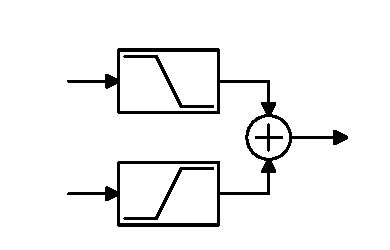
\includegraphics[scale=1]{CF}\\
   % translate x=376 y=304 scale 0.38
   \putbox{1.01in}{1.26in}{1.20}{\centbox{LPF}}%
   \putbox{1.01in}{0.51in}{1.20}{\centbox{HPF}}%
   \putbox{0.35in}{1.12in}{1.20}{\centbox{\midbox{$x_1$}}}%
   \putbox{0.35in}{0.39in}{1.20}{\centbox{\midbox{$x_2$}}}%
   \putbox{2.16in}{0.81in}{1.20}{\centbox{\midbox{$y$}}}%
   } % close 'parbox'
   } % close 'scalebox'
   \vspace{-\baselineskip} % this is not necessary, but looks better

\caption{Filtro complementario.}
\label{fig:CF}
\end{figure}

El filtro pasa bajo y el filtro pasa altos tienen la misma 
frecuencia de corte \( \omega_c \).

Para utilizar el filtro complementario en la medición del 
ángulo de inclinación se utiliza el esquema de la 
Figura~\ref{fig:CFaccgyro}.

\begin{figure}[h!tb]
\centering
% XCircuit output "CFaccgyro.tex" for LaTeX input from CFaccgyro.ps
\def\putbox#1#2#3#4{\makebox[0in][l]{\makebox[#1][l]{}\raisebox{\baselineskip}[0in][0in]{\raisebox{#2}[0in][0in]{\scalebox{#3}{#4}}}}}
\def\rightbox#1{\makebox[0in][r]{#1}}
\def\centbox#1{\makebox[0in]{#1}}
\def\topbox#1{\raisebox{-0.60\baselineskip}[0in][0in]{#1}}
\def\midbox#1{\raisebox{-0.20\baselineskip}[0in][0in]{#1}}
   \scalebox{1}{
   \normalsize
   \parbox{4.04167in}{
   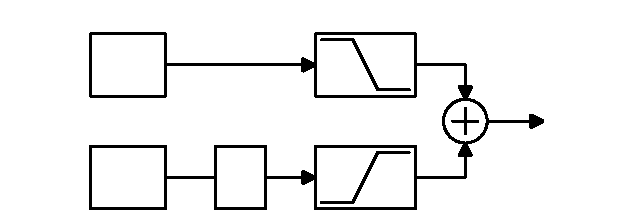
\includegraphics[scale=1]{CFaccgyro}\\
   % translate x=649 y=304 scale 0.38
   \putbox{1.60in}{0.26in}{1.20}{\centbox{\midbox{$\int$}}}%
   \putbox{2.44in}{1.26in}{1.20}{\centbox{LPF}}%
   \putbox{2.44in}{0.51in}{1.20}{\centbox{HPF}}%
   \putbox{0.85in}{1.10in}{1.20}{\centbox{\midbox{$\theta_m$}}}%
   \putbox{0.85in}{0.93in}{1.20}{\centbox{\midbox{Accel}}}%
   \putbox{0.85in}{0.18in}{1.20}{\centbox{\midbox{Gyro}}}%
   \putbox{0.85in}{0.35in}{1.20}{\centbox{\midbox{$\dot{\theta}_m$}}}%
   \putbox{3.58in}{0.79in}{1.20}{\centbox{\midbox{$\theta_e$}}}%
   } % close 'parbox'
   } % close 'scalebox'
   \vspace{-\baselineskip} % this is not necessary, but looks better

\caption{Filtro complementario.}
\label{fig:CFaccgyro}
\end{figure}

Mezclando las funciones de transferencia obtenidas 
 anteriormente se llega la siguiente función de transferencia 
para el filtro

\[ \theta_e(z) = \frac{\omega_c}{(1-z^{-1})/T_0 + \omega_c} \theta_m (z) + \frac{T_0}{1-z^{-1}} \frac{(1-z^{-1})/T_0}{(1-z^{-1})/T_0 + \omega_c} \dot{\theta}_m(z) \]

Simplificando esta función de transferencia se llega a
\[ \theta_e(z) = \frac{\omega_c}{(1-z^{-1})/T_0 + \omega_c} \theta_m (z) + \frac{1}{(1-z^{-1})/T_0 + \omega_c} \dot{\theta}_m(z) \]

Reordenando

\[ \theta_e(z)\left[ (1-z^{-1})/T_0 + \omega_c \right] = 
\omega_c \theta_m(z) + \dot{\theta}_m(z) \]

Aplicando transformada Z inversa
\begin{align*}
\theta_e(k)(1/T_0 + \omega_c) &= \theta_e(k-1)/T_0 + \omega_c \theta_m(k) + \dot{\theta}_m(k) \\
\theta_e(k) &= \frac{1/T_0}{1/T_0 + \omega_c} \theta_e(k-1) 
				+ \frac{1}{1/T_0 + \omega_c} \dot{\theta}_m(k) 
				+ \frac{\omega_c}{1/T_0 + \omega_c} \theta_m(k) \\
				&= \frac{1/T_0}{1/T_0 + \omega_c}[\theta_e(k-1) 
				+ T_0 \dot{\theta}_m(k) ]
				+ \frac{\omega_c}{1/T_0 + \omega_c} \theta_m(k)  \\
				&= (1-\alpha)[\theta_e(k-1) + T_0 \dot{\theta}_m(k) ] + \alpha \theta_m(k)
\end{align*}

Resultado de aplicar el filtro complementario
\begin{figure}[h!tb]
\centering
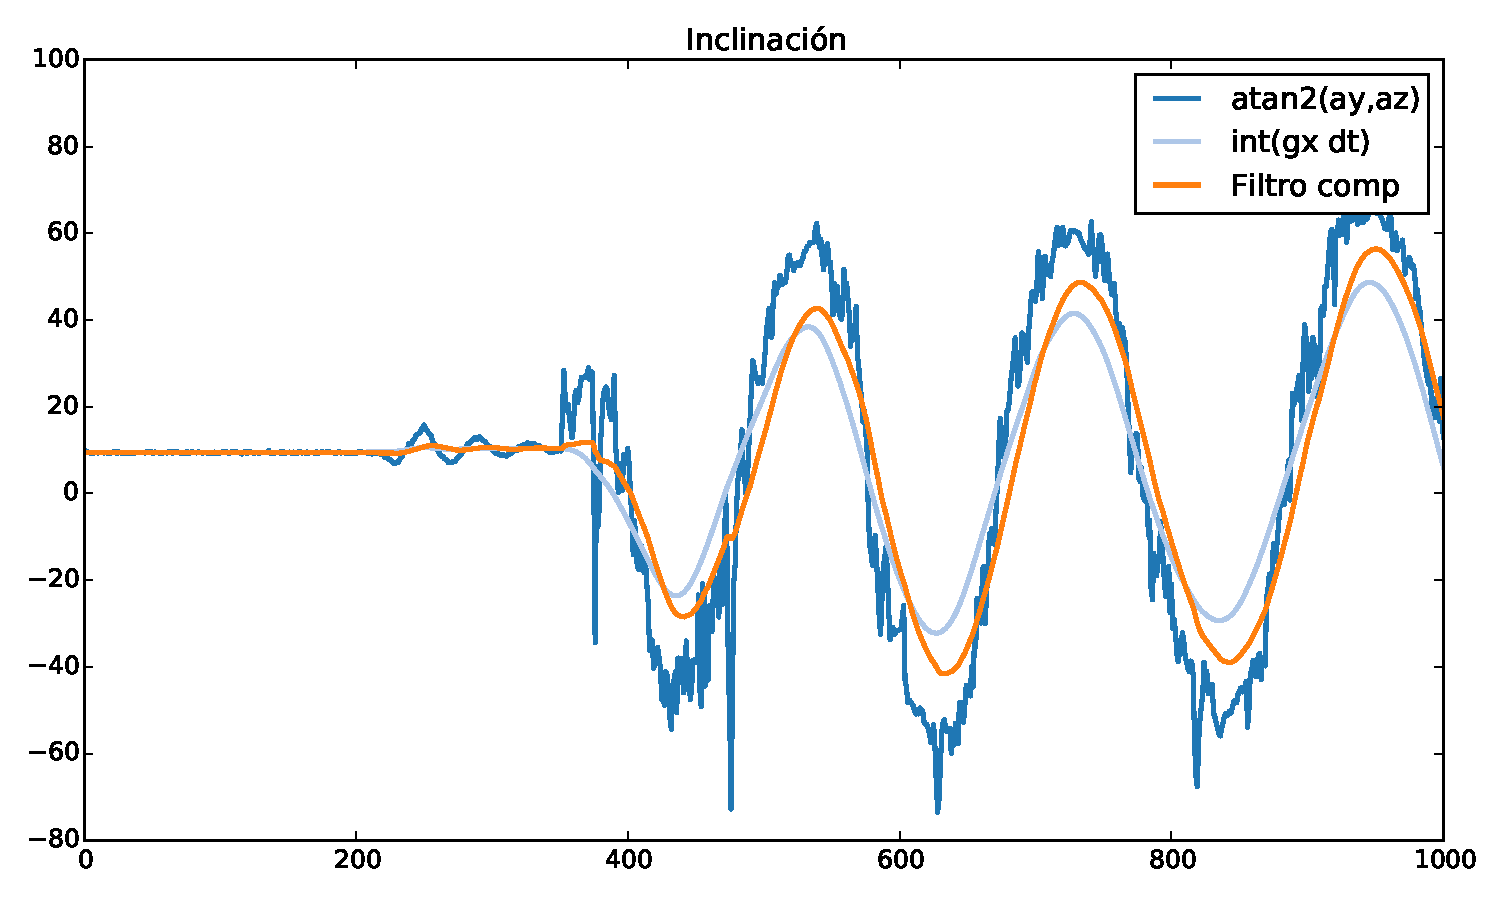
\includegraphics[width=0.9\linewidth]{tilt}
\caption{Ángulo de inclinación usando filtro complementario.}
\label{fig:comp_filt}
\end{figure}

\end{document}
